\section{Software Requirements}
\begin{itemize}
    \item {MATLAB}
    \item {Simulink}
\end{itemize}

\section{Hardware Requirements}
Following are the required components:
\begin{itemize}
    \item {Induction motor.}
    \item {Arduino UNO.}
    \item {Condition monitoring Sensors (Like Voltage transformer, Current transformer, Speed sensor)}
    \item {Speed controlling Device.}
    \item {Gate Driver Circuit.}
    \item {LCD}
    \item {ESP8266(WIFI Module).}
\end{itemize}

\section{Induction Motor}
The induction motor is known as an asynchronous motor. The induction motor has its advantages like its necessary characteristic, robustness, and effectiveness than any other type of Motor. Here in our project, induction motor plays a significant role.\\
Parameters:\\
Volts-415v \\
Frequency- 50Hz\\
Speed- 1440 rpm\\
{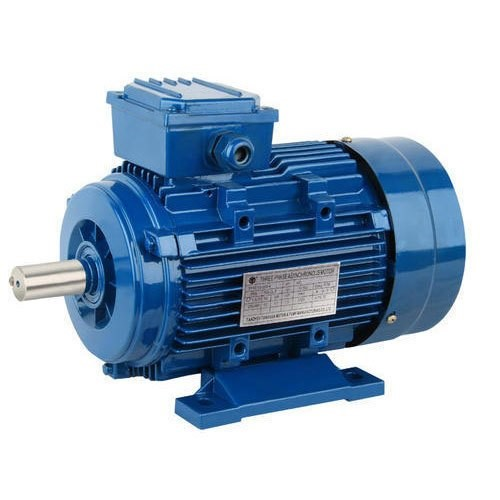
\includegraphics[height=0.2\textheight]{Figures/motor.jpg}}

\section{Arduino UNO}
Arduino Uno is a low-cost, flexible, and easy-to-use programmable open-source microcontroller board that can be integrated into various electronic projects. This board can be interfaced with other Arduino boards, Arduino shields, Raspberry Pi boards and can control relays, LEDs, servos, and motors as an output.\\
{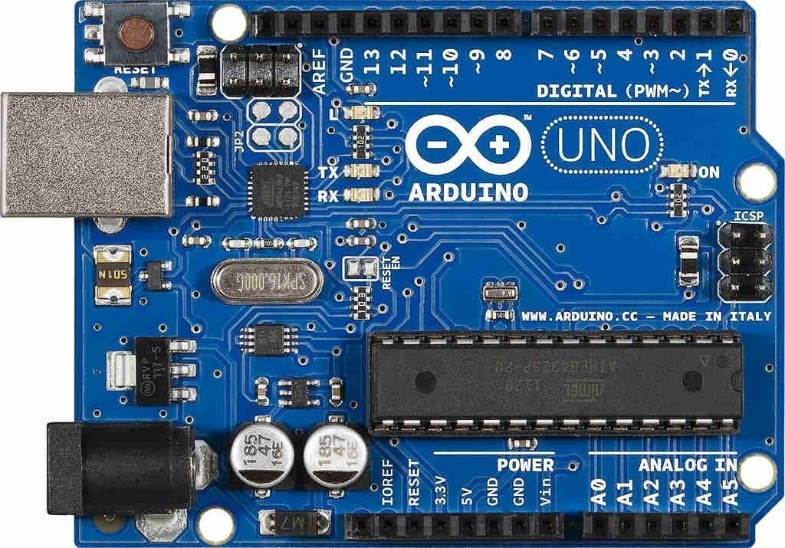
\includegraphics[height=0.2\textheight]{Figures/arduino.jpg}}

\section{Conditional Monitoring Sensor}
There are three sensors used for monitoring and evaluation management in the system.\\
\begin{itemize}
    \item {We use a voltage transformer to measure the supply voltage as it acts as a step-down and sensing of the supply voltage.}
    \item {Current transformer for measuring motor current}
    \item {IR Sensor for measuring speed}
\end{itemize}
\subsection{Voltage Transformer}
The voltage transformer is used for measuring high alternating voltage purposes; here in this project, it also acts as a sensor for sensing the supply voltage of an Induction Motor. It is a step-down transformer that converts 230 v to 4 v supply.\\
{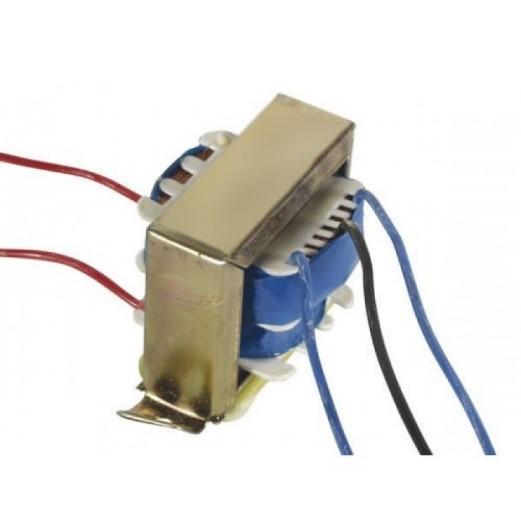
\includegraphics[height=0.2\textheight]{Figures/volt.jpg}}
\section{Current Transformer}
The current transformer is used to measure high alternating current, and here it also acts as a sensor for sensing the current that flows in the Induction Motor. It has an input current rating of 5A, and an analogy output current rating is 5mA. It is a 5A range of single-phase AC sensor modules. It has a 1000: 1 turn ratio.\\
{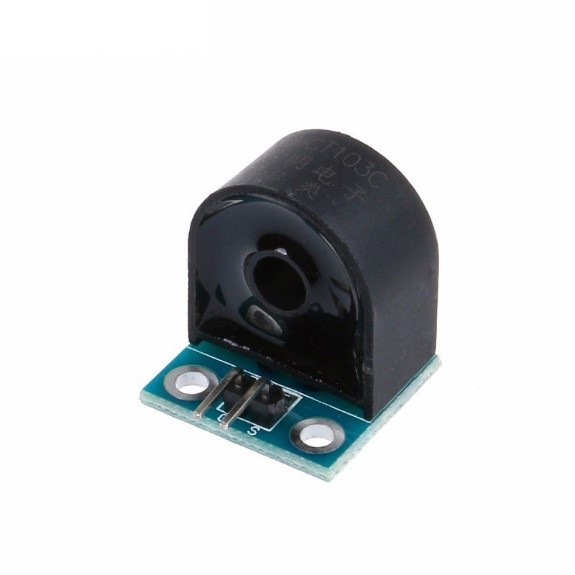
\includegraphics[height=0.2\textheight]{Figures/trans.jpg}}
\subsection{IR Sensor Module}
It is an electronic device to measure and detect infrared radiation from its surrounding atmosphere. It includes LED and an infrared laser diode. It works as a digital tachometer. IR sensor used for measuring the speed of 3 phase Induction Motor in rpm. It has an operating voltage that is 3 to 5v.\\
{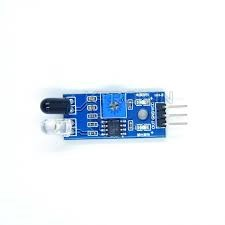
\includegraphics[height=0.2\textheight]{Figures/ir.jpg}}
\subsection{Speed Controlling Device}
BT139 Triac is a semiconductor device with a plastic envelope packaged, high bidirectional transistor, and high blocking voltage capability. BT139 is a Triac switch used for the speed controlling purpose of an induction motor with the help of the gate triggering circuit. The gate driver circuit is for logical purposes to operate the Triac switch.\\
{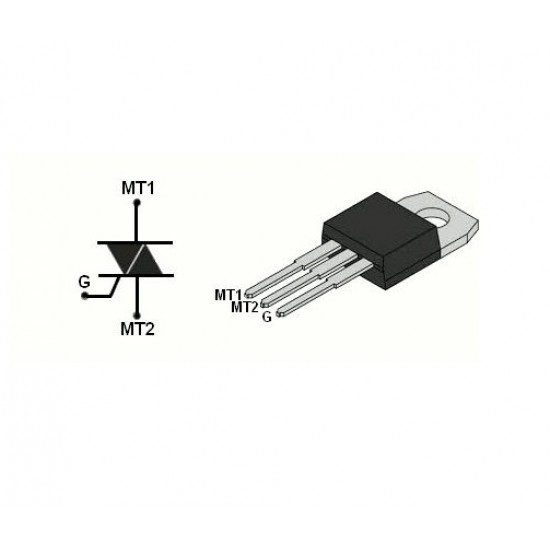
\includegraphics[height=0.2\textheight]{Figures/triac.jpg}}
\subsection{LCD Display}
LCD is an electronic screen display module. The type of LCD used in this proposed system for continuously displaying the monitored value of an induction motor is 16x4. Here 16 values indicate the character on a single line, and four indicate the number of lines. Operation of LCD requires a 5V DC supply.\\
{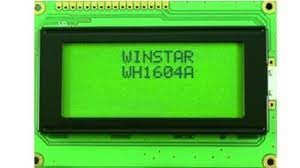
\includegraphics[height=0.2\textheight]{Figures/lcd.jpg}}
\subsection{ESP8266}
We use the Wi-Fi module for communication with the cloud. We have used the ESP8266 Wi-Fi module to exchange information between devices to the cloud without connecting to any wire. Each device has its I.P address. For connection to the cloud,  the I.P address is entered on the Android application, and the devices in the system, i.e., induction motor, sensors, speed controlling device. 
These are connected to the cloud and send information to the cloud without any wired connection, i.e., through the Wi-Fi module send information for further process.
{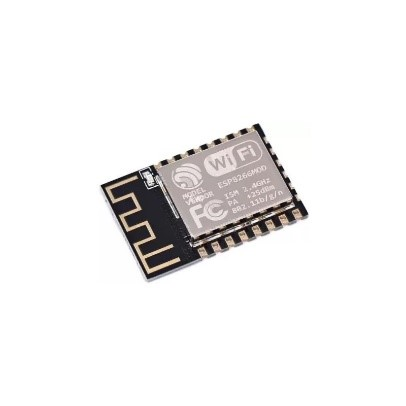
\includegraphics[height=0.2\textheight]{Figures/esp.jpg}}

\section{Block Diagram}
{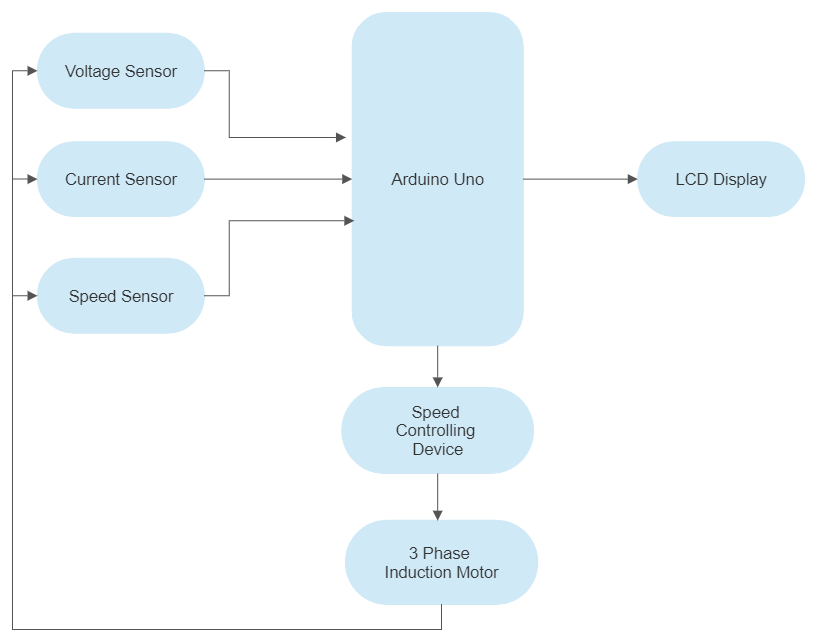
\includegraphics[height=0.5\textheight]{Figures/Drawing.jpg}}

\section{Method}
3 phase AC supply comes into the system; from AC supply to 3 phase Induction Motor through a speed controlling device and gate driver circuit. Here, the gate driver circuit acts as a logic circuit to on-off the switches to control the motor's speed. There are many methods to control the speed of the motor, but the PWM technique has been used here to control the speed of an induction motor. PWM technique is very sophisticated to use and most sophisticated to operate than any other method. By adjusting the ON-OFF period of TRIAC switches controlling the firing angle and, from that, the firing angle controls the speed of the induction motor.




